
%\chapter{Background and related work}
\chapter{Background} \label{chap:background}

    In order to understand and construct a framework capable of solving a wide variety of matching problems, it is essential to first explore the theoretical foundations that support this approach. This chapter presents the key concepts necessary for modeling, analyzing, and solving grouping problems in industry.

    We begin by introducing basic elements from graph theory, which is the foundation for representing entities and relationships in matching problems. Then, we explore the formal concept of matching, including fairness constraints and cost optimization using flow networks. To complement this, we review the set cover problem, which offers a broader perspective on grouping scenarios that go beyond pairwise relations.

    As the proposed solution is designed to be adaptable to real-world software systems, we also introduce the concept of Object-Relational Mapping (ORM), a widely used modeling paradigm in the software industry. This allows the framework to be integrated directly with relational data models in existing applications.

    Finally, we present an overview of genetic algorithms, a class of metaheuristics suitable for solving complex optimization problems where exact methods may be infeasible. These algorithms will later be applied as solvers within the proposed framework.

Together, these concepts provide the theoretical and practical basis for the design and implementation of the categorised grouping framework developed in this dissertation.
    \section{Graphs}
    
        Graphs are a fundamental concept in computer science and mathematics, widely used to represent relationships between objects. A graph \( G \) is defined as a pair \( (V, E) \), where \( V \) is a set of vertices (or nodes) and \( E \) is a set of edges \cite{cormen}. Each edge in \( E \) connects a pair of vertices.

        \subsection{Vertices and Edges}
        
            The primary components of a graph are vertices and edges \cite{cormen, bondy1976graph}. A vertex (singular of vertices) represents a discrete entity in the graph, often denoted as \( v \in V \). An edge connects two vertices and represents the relationship between them. An edge is typically denoted as \( e = (u, v) \in E \), where \( u, v \in V \).
            %
            In Figure \ref{fig:base_graph}, the vertices are represented as circles and the edges are represented as lines.

            
            \begin{figure}[!ht]
                \centering
                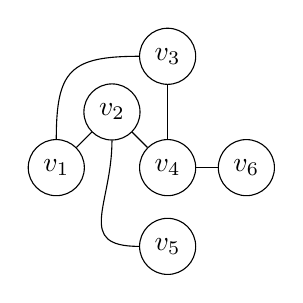
\begin{tikzpicture}[main/.style = {draw, circle}] 
                    \node[main] (1) {$v_1$};
                    \node[main] (2) [above right of=1] {$v_2$};
                    \node[main] (3) [above right of=2] {$v_3$}; 
                    \node[main] (4) [below right of=2] {$v_4$};
                    \node[main] (5) [below of=4] {$v_5$};
                    \node[main] (6) [right of=4] {$v_6$};

                    \draw (2) -- (4);
                    \draw (1) -- (2);
                    \draw (4) -- (3);
                    \draw (4) -- (6);
                    \draw (1) to [out=90,in=180,looseness=1.5] (3);
                    \draw (2) to [out=270,in=180,looseness=1.5] (5);
                \end{tikzpicture}
                \caption[Graph $G = (V, E)$.]{Graph $G = (V, E)$. The circles ($v_1, \ldots, v_6$) are the vertices $V$; the lines connecting the vertices are the edges $E$.} \label{fig:base_graph}
            \end{figure}
        
        \subsection{Subgraphs}
        
            A subgraph \( G' \) of a graph \( G \) is a graph formed from a subset of the vertices and edges of \( G \) \cite{cormen, bondy1976graph}. Formally, \( G' = (V', E') \) is a subgraph of \( G = (V, E) \) if \( V' \subseteq V \) and \( E' \subseteq E \). Figure \ref{fig:subgraphs} provide examples of subgraphs of Graph G presented in Figure \ref{fig:base_graph}.

            \begin{figure}[!ht]
                \centering
                \begin{subfigure}{0.24\textwidth}
                    \centering
                    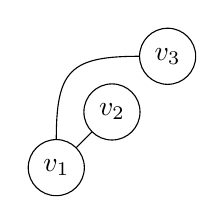
\begin{tikzpicture}[main/.style = {draw, circle}] 
                        \node[main] (1) {$v_1$};
                        \node[main] (2) [above right of=1] {$v_2$};
                        \node[main] (3) [above right of=2] {$v_3$}; 

                
                        \draw (1) -- (2);
                        \draw (1) to [out=90,in=180,looseness=1.5] (3);
                    \end{tikzpicture}
                    \caption{Subgraph $G_1$} 
                    \label{fig:subgraph_1}
                \end{subfigure}
                \hfill
                \begin{subfigure}{0.24\textwidth}
                    \centering
                    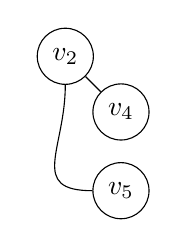
\begin{tikzpicture}[main/.style = {draw, circle}] 
                        \node[main] (2) {$v_2$};
                        \node[main] (4) [below right of=2] {$v_4$};
                        \node[main] (5) [below of=4] {$v_5$};
                
                        \draw (2) -- (4);
                        \draw (2) to [out=270,in=180,looseness=1.5] (5);
                    \end{tikzpicture}
                    \caption{Subgraph $G_2$} 
                    \label{fig:subgraph_2}
                \end{subfigure}
                \hfill
                \begin{subfigure}{0.24\textwidth}
                    \centering
                    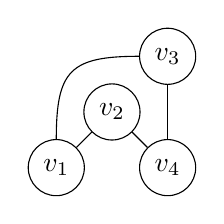
\begin{tikzpicture}[main/.style = {draw, circle}] 
                        \node[main] (1) {$v_1$};
                        \node[main] (2) [above right of=1] {$v_2$};
                        \node[main] (3) [above right of=2] {$v_3$}; 
                        \node[main] (4) [below right of=2] {$v_4$};

                        \draw (2) -- (4);
                        \draw (1) -- (2);
                        \draw (4) -- (3);
                        \draw (1) to [out=90,in=180,looseness=1.5] (3);
                    \end{tikzpicture}
                    \caption{Subgraph $G_3$} 
                    \label{fig:subgraph_3}
                \end{subfigure}
                \hfill
                % \begin{subfigure}{0.24\textwidth}
                %     \centering
                %     \begin{tikzpicture}[main/.style = {draw, circle}] 
                %         \node[main] (1) {$v_1$};
                %         \node[main] (2) [above right of=1] {$v_2$};
                %         \node[main] (3) [above right of=2] {$v_3$}; 
                %         \node[main] (4) [below right of=2] {$v_4$};

                %         \draw (2) -- (4);
                %         \draw (1) -- (2);
                %         \draw (4) -- (3);
                %     \end{tikzpicture}
                %     \caption{Subgraph $G_4$} 
                %     \label{fig:subgraph_4}
                % \end{subfigure}
                \caption{Three possible subgraphs of Graph $G$ (See Figure \ref{fig:base_graph}).}
                \label{fig:subgraphs}
            \end{figure}
        
        \subsection{Subsets of Vertices}
        
            Subsets of vertices play a crucial role in various graph algorithms and properties \cite{cormen, bondy1976graph}. Given a graph \( G = (V, E) \), a subset of vertices \( S \subseteq V \) can be used to define induced subgraphs, vertex covers, and other structures. For example, the induced subgraph \( G[S] \) is formed by the vertices in \( S \) and all the edges between them in \( G \). Figure \ref{fig:subset_of_vertices} shows a subset of vertices of $G_2$ (See Figure \ref{fig:subgraph_2}).

            \begin{figure}[!ht]
                \centering
                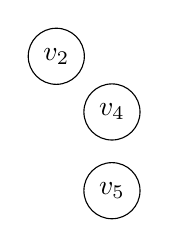
\begin{tikzpicture}[main/.style = {draw, circle}] 
                    \node[main] (2) {$v_2$};
                    \node[main] (4) [below right of=2] {$v_4$};
                    \node[main] (5) [below of=4] {$v_5$};
                \end{tikzpicture}
                \caption[Subset of vertices from Graph $G$.]{Subset of vertices from Graph $G$ (Figure \ref{fig:base_graph}) which induces (generates) the Graph $G''$ (Figure \ref{fig:subgraph_2}).}
                \label{fig:subset_of_vertices}
            \end{figure}


        \subsection{Bipartite Graphs}

            A bipartite graph is a graph \( G = (V, E) \) whose vertices can be divided into two disjoint sets \( V_1 \) and \( V_2 \) such that every edge in \( E \) connects a vertex in \( V_1 \) to a vertex in \( V_2 \) \cite{cormen, bondy1976graph}.
            Formally, a graph \( G \) is bipartite if \( V \) can be partitioned into two sets \( V_1 \) and \( V_2 \) such that \( V_1 \cap V_2 = \emptyset \) and every edge in \( E \) has one endpoint in \( V_1 \) and the other in \( V_2 \). Figure \ref{fig:G_bipartite_by_layer} depics examples of bipartite graphs and Figure \ref{fig:non_bipartite_graph} shows an example of a non-bipartite graph.
            
            Bipartite graphs have many applications in various fields, including computer science, biology, and social sciences. They are used to model relationships between two different classes of objects, such as students and courses, users and items, or proteins and genes. 
            %
            One common algorithmic problem on bipartite graphs is the maximum bipartite matching problem, which aims to find the largest subset of edges in the graph such that no two edges share a common vertex.
            
        \begin{figure}[!ht]
            \centering
            \begin{subfigure}{0.3\textwidth}
                \centering
                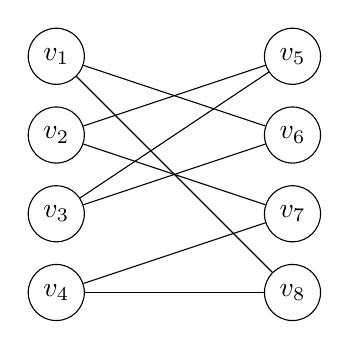
\begin{tikzpicture}[main/.style = {draw, circle}] 
                    \node[main] (1) {$v_1$};
                    \node[main] (2) [below of=1] {$v_2$};
                    \node[main] (3) [below of=2] {$v_3$};
                    \node[main] (4) [below of=3] {$v_4$};
        
                    \node[main] (5) [right of=1, xshift=2cm]{$v_5$};
                    \node[main] (6) [below of=5] {$v_6$};
                    \node[main] (7) [below of=6] {$v_7$};
                    \node[main] (8) [below of=7] {$v_8$};
        
                    \draw (1) -- (8);
                    \draw (1) -- (6);
                    \draw (2) -- (5);
                    \draw (2) -- (7);
                    \draw (3) -- (5);
                    \draw (3) -- (6);
                    \draw (4) -- (7);
                    \draw (4) -- (8);
                \end{tikzpicture}
                \caption{}
                \label{fig:common_representation_of_bipartition}
            \end{subfigure}
            \hfill
            \begin{subfigure}{0.3\textwidth}
                \centering
                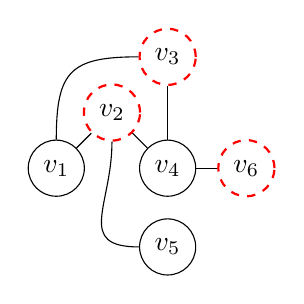
\begin{tikzpicture}[main/.style = {draw, circle}, rednode/.style={draw=red, thick, dashed, circle}] 
                    \node[main] (1) {$v_1$};
                    \node[rednode] (2) [above right of=1] {$v_2$};
                    \node[rednode] (3) [above right of=2] {$v_3$}; 
                    \node[main] (4) [below right of=2] {$v_4$};
                    \node[main] (5) [below of=4] {$v_5$};
                    \node[rednode] (6) [right of=4] {$v_6$};

        
                    \draw (2) -- (4);
                    \draw (1) -- (2);
                    \draw (4) -- (3);
                    \draw (4) -- (6);
                    \draw (1) to [out=90,in=180,looseness=1.5] (3);
                    \draw (2) to [out=270,in=180,looseness=1.5] (5);
                \end{tikzpicture}
                \caption{}
                \label{fig:bipartition_by_color}
            \end{subfigure}
            \hfill
            \begin{subfigure}{0.3\textwidth}
                \centering
                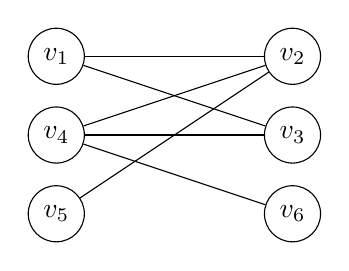
\begin{tikzpicture}[main/.style = {draw, circle}] 
                    \node[main] (1) {$v_1$};
                    \node[main] (4) [below of=1] {$v_4$};
                    \node[main] (5) [below of=4] {$v_5$};
                    

                    \node[main] (2) [right of=1, xshift=2cm]{$v_2$};
                    \node[main] (3) [below of=2] {$v_3$};
                    \node[main] (6) [below of=3] {$v_6$};
                    
        
                    \draw (2) -- (4);
                    \draw (1) -- (2);
                    \draw (4) -- (3);
                    \draw (1) -- (3);
                    \draw (2) -- (5);
                    \draw (4) -- (6);
                \end{tikzpicture}
                \caption{}
                \label{fig:G_bipartite_by_layer}
            \end{subfigure}
            \caption[Examples of bipartite graphs and ways to represent it.]{Examples of bipartite graphs and ways to represent it. (a) Common representation of a bipartite graph (by layer). (b-c) the same Graph $G$ (See Figure \ref{fig:base_graph}), with different bipartite representations. (b) Representation by color, black / solid nodes represent one partition and red / dashed nodes represent the other partition. (c) Representation by layer.}
        \end{figure}

        It is important to note that not every graph is bipartite. A graph that contains an odd-length cycle cannot be bipartite, as it is impossible to partition the vertices into two sets without having two vertices of the same set being adjacent. For example, consider the following graph:
        
        \begin{figure}[!ht]
            \centering
            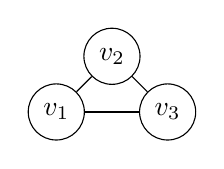
\begin{tikzpicture}[main/.style = {draw, circle}] 
                \node[main] (1) {$v_1$};
                \node[main] (2) [above right of=1] {$v_2$};
                \node[main] (3) [below right of=2] {$v_3$}; 
        
                \draw (1) -- (2);
                \draw (2) -- (3);
                \draw (3) -- (1);
            \end{tikzpicture}
            \caption{Example of a non-bipartite graph.} 
            \label{fig:non_bipartite_graph}
        \end{figure}
        
        This graph contains a cycle of length 3 (vertices \(v_1\), \(v_2\), and \(v_3\)), which is an odd-length cycle. Therefore, it is not possible to divide the vertices into two sets where all edges connect vertices from different sets, making this graph non-bipartite.
        
        \section{Matching}

            A matching (strictly in the context of graph theory) in a graph \( G = (V, E) \) is a set of edges \( M \subseteq E \) such that no two edges in \( M \) share a common vertex \cite{cormen, bondy1976graph}. Matchings are used to model relationships in various applications, such as assigning tasks to workers or pairs in social networks. Figure \ref{fig:possible_matching} shows a possible matching of Graph G (see Figure \ref{fig:base_graph}).
            
            In a bipartite graph, a matching (also called bipartite matching) is a subset of edges \( M \subseteq E \) such that each vertex is incident to at most one edge in \( M \). Finding a maximum matching in a bipartite graph can be efficiently solved using algorithms like the Hopcroft-Karp algorithm \cite{west2001introduction, diestel2017graph}.


            \begin{figure}[!ht]
                \centering
                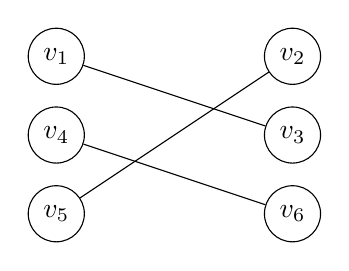
\begin{tikzpicture}[main/.style = {draw, circle}] 
                    \node[main] (1) {$v_1$};
                    \node[main] (4) [below of=1] {$v_4$};
                    \node[main] (5) [below of=4] {$v_5$};
                    

                    \node[main] (2) [right of=1, xshift=2cm]{$v_2$};
                    \node[main] (3) [below of=2] {$v_3$};
                    \node[main] (6) [below of=3] {$v_6$};
                    
        
                    \draw (1) -- (3);
                    \draw (2) -- (5);
                    \draw (4) -- (6);
                \end{tikzpicture}
                \caption{Possible matching of Graph $G$ (see Figure \ref{fig:base_graph}).}
                \label{fig:possible_matching}
            \end{figure}
            
        \subsection{Bipartite Matching}

            Bipartite Matching, also known as bipartite pairing is a fundamental problem in graph theory, with many practical applications, including resource allocation, market design, and job assignment.
            We have two distinct sets of elements, and the objective is to find corresponding pairs between them while also optimizing some criteria.
            
            To formalize the problem, consider a graph \( G = (V, E) \), where the vertex set \( V \) is partitioned into two disjoint subsets \( V_1 \) and \( V_2 \), such that \( V = V_1 \cup V_2 \) and \( V_1 \cap V_2 = \emptyset \). The goal is to identify a set of edges \( M \subseteq E \) that connect vertices from \( V_1 \) to \( V_2 \), ensuring that no two edges in \( M \) share a common vertex. This configuration is commonly referred to as a \textit{matching} \cite{hopcroft1973n}.
            
            It is important to note that in some cases, sets have different sizes, and thus it is not possible to match every vertex of both sets.
            
        \subsection{Fairness in Matching}
            
            Fairness in matching consists in take into account specific attributes of the set of vertices and their proportionality in the solution.
            %%
            Inspired by the work of \cite{sankar}, the notion of fairness adopted by this study is delegated to an external operator. This impartial operator does not directly engage with the sets being matched. Instead, it has the responsibility to judge the fairness in the matching context.
            
            In the search for pairing a set $U$ and a set $V$, the concept of giving priority to some specific subset of $U$ that contains specific traits is proposed. This different approach to the original problem is particularly relevant in scenarios where prioritizing different characteristics alongside minimal cost is desired.
            
            To operationalize this prioritization, this work employs the concept of minimum quotas, which establish a minimum number of vacancies reserved for specific subsets. 
            These minimum quotas, act as instruments to promote equity in the matching process, ensuring those specific subsets receive adequate representation.
            
            The quotas refer to the predetermined allocation of a minimum number of matchings to each special subset, thereby establishing a fair distribution of pairings. This definition is crucial for ensuring representativity and preventing imbalances in the allocations.
            
            It is important to highlight that, in this study, the quotas are only applied to one set of the bipartite graph, meaning that only $U$ or $V$ is involved in the quota implementation.
            
            This definition of quotas aligns with the fairness proposed by \cite{sankar}, where the imposition of quotas becomes essential to maximize equity in the resources allocated. The next session approaches how this definition of fairness is represented in the mapping to the MCMF problem. 
            
        \subsection{Minimum Cost Maximum Flow}
            
            The minimum cost maximum flow problem refers to the search for the maximum amount of possible flow in a network, considering costs associated with the passage of flow through certain uniderected edges \cite{korte2018combinatorial, ford1956maximal}. In other words, the objective of such problems is to optimize the transportation of resources from one point to another while minimizing the costs involved in this process.
            
            This concept has broad applications, often used in transportation problems, network design, and linear programming, among others. Efficient resolution of Minimum-Cost Maximum Flow (MCMF) problems is crucial in various fields, contributing to the efficiency and economy of resources.
            
        \subsection{Solving Bipartite Matching with MCMF}\label{subsubsec:resolucao-fluxo-matching}
            
            To clarify the methodology of mapping a Bipartite Matching problem to a Minimum-Cost Maximum Flow (MCMF) problem, a method that is already well-known and documented \cite{ahuja1993network, edmonds1972theoretical, tarjan1997dynamic}, we present a detailed visual representation of this process in Figure~\ref{fig:mcmf}.
            %%
            % In this bipartite graph, the sets of nodes $U$ and $V$. 
            In this figure, the bipartite graph being matched is the set of nodes $U = \{u_1, \ldots, u_6\}$ (in red/dashed) and $V = \{v_1, \ldots, v_3\}$ (in blue/dotted). 
            %The edges connecting these sets have two parameters: the first number denotes the capacity, indicating the maximum number of flows that can be assigned to a given task, while the second number represents the cost associated with the edge. 
            The edges connecting the sets $U$ and $V$ have two parameters ($K;C$): the first parameter $K$, denotes the capacity, indicating the maximum number of flows that can be assigned to a given task, while the second parameter $C$, represents the cost associated with the edge. 

            The mapping strategy involves representing the bipartite graph as a flow network. 
            Two other nodes are added, a Source, connected to all nodes in Set $U$, and a Sink, connected to all nodes in Set $V$. 
            It is worth noting that the edges connected to the Source and Sink sets have zero cost and unit capacity ($1;0$) to guarantee that the added connections do not affect the overall cost minimization.
            
            \begin{figure}[ht] \centering
                \resizebox{0.5\textwidth}{!}{%
 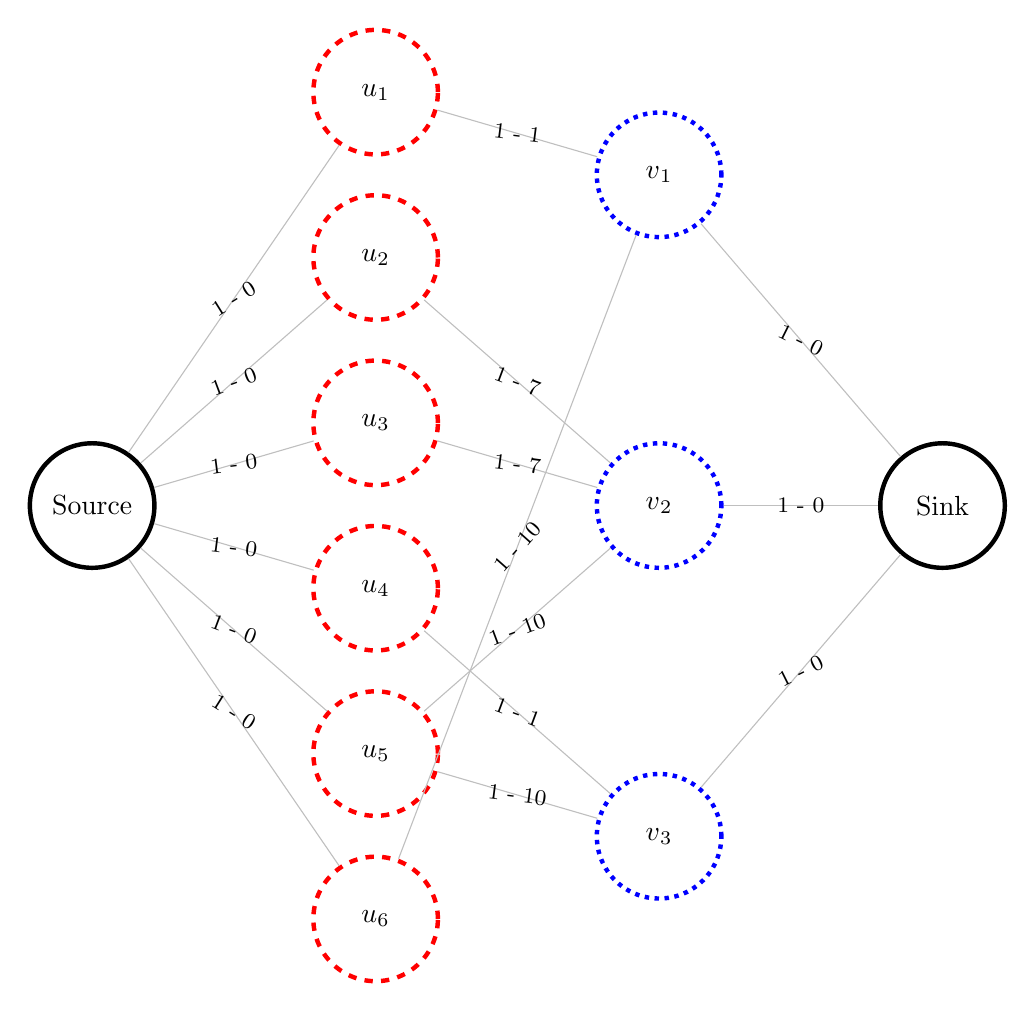
\begin{tikzpicture}[xscale=0.45,yscale=1.05]
   \tikzstyle{style} = [circle, draw, ultra thick, minimum size=45pt, inner sep=0pt, text centered]


      \draw
        (-10.909, 0.0) node[style, draw=black] (0){Source}
        (-2.909, 5.0) node[style, draw=red, dashed] (1){$u$$_1$}
        (-2.909, 3.0) node[style, draw=red, dashed] (2){$u$$_2$}
        (-2.909, 1.0) node[style, draw=red, dashed] (3){$u$$_3$}
        (-2.909, -1) node[style, draw=red, dashed] (4){$u$$_4$}
        (-2.909, -3.0) node[style, draw=red, dashed] (5){$u$$_5$}
        (-2.909, -5.0) node[style, draw=red, dashed] (6){$u$$_6$}
        (5.091, 4) node[style, draw=blue, dotted] (7){$v$$_1$}
        (5.091, -4.0) node[style, draw=blue, dotted] (8){$v$$_3$}
        (5.091, 0) node[style, draw=blue, dotted] (9){$v$$_2$}
        (13.091, 0.0) node[style, draw=black] (10){Sink};

  %   \tikzstyle{style} = [circle, draw, fill, minimum size=45pt, inner sep=0pt, text centered]


      % \draw
      %   (-10.909, 0.0) node[style, fill=cyan] (0){Source}
      %   (-2.909, 5.0) node[style, fill=brown] (1){$u$$_1$}
      %   (-2.909, 3.0) node[style, fill=brown] (2){$u$$_2$}
      %   (-2.909, 1.0) node[style, fill=brown] (3){$u$$_3$}
      %   (-2.909, -1) node[style, fill=brown] (4){$u$$_4$}
      %   (-2.909, -3.0) node[style, fill=brown] (5){$u$$_5$}
      %   (-2.909, -5.0) node[style, fill=brown] (6){$u$$_6$}
      %   (5.091, 4) node[style, fill=orange] (7){$v$$_1$}
      %   (5.091, -4.0) node[style, fill=orange] (8){$v$$_3$}
      %   (5.091, 0) node[style, fill=orange] (9){$v$$_2$}
      %   (13.091, 0.0) node[style, fill=cyan] (10){Sink};
    
  \begin{scope}[-]
    \draw[lightgray, text=black, font=\footnotesize] (0) to node[midway, sloped, ] {1 - 0} (1);
    \draw[lightgray, text=black, font=\footnotesize] (0) to node[midway, sloped, ] {1 - 0} (2);
    \draw[lightgray, text=black, font=\footnotesize] (0) to node[midway, sloped, ] {1 - 0} (3);
    \draw[lightgray, text=black, font=\footnotesize] (0) to node[midway, sloped, ] {1 - 0} (4);
    \draw[lightgray, text=black, font=\footnotesize] (0) to node[midway, sloped, ] {1 - 0} (5);
    \draw[lightgray, text=black, font=\footnotesize] (0) to node[midway, sloped, ] {1 - 0} (6);
    \draw[lightgray, text=black, font=\footnotesize] (1) to node[midway, sloped, ] {1 - 1} (7);
    \draw[lightgray, text=black, font=\footnotesize] (2) to node[midway, sloped, ] {1 - 7} (9);
    \draw[lightgray, text=black, font=\footnotesize] (3) to node[midway, sloped, ] {1 - 7} (9);
    \draw[lightgray, text=black, font=\footnotesize] (4) to node[midway, sloped, ] {1 - 1} (8);
    \draw[lightgray, text=black, font=\footnotesize] (5) to node[midway, sloped, ] {1 - 10} (9);
    \draw[lightgray, text=black, font=\footnotesize] (5) to node[midway, sloped, ] {1 - 10} (8);
    \draw[lightgray, text=black, font=\footnotesize] (6) to node[midway, sloped, ] {1 - 10} (7);
    \draw[lightgray, text=black, font=\footnotesize] (7) to node[midway, sloped, ] {1 - 0} (10);
    \draw[lightgray, text=black, font=\footnotesize] (8) to node[midway, sloped, ] {1 - 0} (10);
    \draw[lightgray, text=black, font=\footnotesize] (9) to node[midway, sloped, ] {1 - 0} (10);
  \end{scope}
\end{tikzpicture}
}%
                \caption{Mapping of bipartite matching to flow problem.}
                \label{fig:mcmf} 
            \end{figure}
            
            \begin{figure}[ht] \centering 
                
  % \begin{tikzpicture}[scale=0.7]
  %     \draw
  %       (-6.545, 0.0) node[draw=cyan, rounded corners] (0){Source}
  %       (-2.545, 1.2) node[draw=red, dashed, rounded corners] (1){$u$}
  %       (-2.545, 0.0) node[draw=red, dashed, rounded corners] (2){$u$}
  %       (-2.545, -1.2) node[draw=red, dashed, rounded corners] (3){$u$}
  %       (1.455, 3.0) node[draw=blue, dotted, rounded corners] (4){$v$}
  %       (1.455, 1.8) node[draw=blue, dotted, rounded corners] (5){$v$}
  %       (1.455, 0.6) node[draw=blue, dotted, rounded corners] (6){$v$}
  %       (1.455, -0.6) node[draw=blue, dotted, rounded corners] (7){$v$}
  %       (1.455, -1.8) node[draw=blue, dotted, rounded corners] (8){$v$}
  %       (1.455, -3.0) node[draw=blue, dotted, rounded corners] (9){$v$}
  %       (5.455, 0.0) node[draw=cyan, rounded corners] (10){Target};
  %     \begin{scope}[-]
  %       \draw[lightgray, text=black, font=\footnotesize]  (0) to node[]{0} (1);
  %       \draw[lightgray, text=black, font=\footnotesize]  (0) to  node[]{0} (2);
  %       \draw[lightgray, text=black, font=\footnotesize]  (0) to node[]{0}  (3);
  %       \draw[lightgray, text=black, font=\footnotesize]  (1) to  node[]{1} (4);
  %       \draw[lightgray, text=black, font=\footnotesize]  (2) to  node[]{2} (6);
  %       \draw[lightgray, text=black, font=\footnotesize]  (3) to  node[]{4} (9);
  %       \draw[lightgray, text=black, font=\footnotesize]  (4) to  node[]{0} (10);
  %       \draw[lightgray, text=black, font=\footnotesize]  (6) to  node[]{0} (10);
  %       \draw[lightgray, text=black, font=\footnotesize]  (9) to  node[]{0} (10);
  %     \end{scope}
  %   \end{tikzpicture}
    
\resizebox{0.5\textwidth}{!}{%
 \begin{tikzpicture}[xscale=0.45,yscale=1.05]
    \tikzstyle{style} = [circle, ultra thick, draw, draw, minimum size=45pt, inner sep=0pt, text centered]
    \tikzstyle{no_border} = [circle, draw, minimum size=45pt, inner sep=0pt, text centered, opacity=0.5]


      \draw
        (-10.909, 0.0) node[style, draw=black] (0){Source}
        (-2.909, 5.0) node[style, draw=red, dashed] (1){$u$$_1$}
        (-2.909, 3.0) node[style, draw=red, dashed] (2){$u$$_2$}
        (-2.909, 1.0) node[no_border, draw=red, dashed] (3){$u$$_3$}
        (-2.909, -1) node[style, draw=red, dashed] (4){$u$$_4$}
        (-2.909, -3.0) node[no_border, draw=red, dashed] (5){$u$$_5$}
        (-2.909, -5.0) node[no_border, draw=red, dashed] (6){$u$$_6$}
        (5.091, 4) node[style, draw=blue, dotted] (7){$v$$_1$}
        (5.091, -4.0) node[style, draw=blue, dotted] (8){$v$$_3$}
        (5.091, 0) node[style, draw=blue, dotted] (9){$v$$_2$}
        (13.091, 0.0) node[style, draw=black] (10){Sink};
    
      \begin{scope}[->, >=BigLatex]
        \draw[lightgray, text=black, font=\normalsize] (0) to node[] {1 ; 0} (1);
        \draw[lightgray, text=black, font=\normalsize] (0) to node[] {1 ; 0} (2);
        \draw[transparent] (0) to node[] {0 ; 0} (3);
        \draw[lightgray, text=black, font=\normalsize] (0) to node[] {1 ; 0} (4);
        \draw[transparent] (0) to node[] {0 ; 0} (5);
        \draw[transparent] (0) to node[] {0 ; 0} (6);
        \draw[lightgray, text=black, font=\normalsize] (1) to node[] {1 ; 1} (7);
        \draw[lightgray, text=black, font=\normalsize] (2) to node[] {1 ; 7} (9);
        \draw[transparent] (3) to node[] {0 ; 7} (9);
        \draw[lightgray, text=black, font=\normalsize] (4) to node[] {1 ; 1} (8);
        \draw[transparent] (5) to node[] {0 ; 10} (9);
        \draw[transparent] (5) to node[] {0 ; 10} (8);
        \draw[transparent] (6) to node[] {0 ; 10} (7);
        \draw[lightgray, text=black, font=\normalsize] (7) to node[] {1 ; 0} (10);
        \draw[lightgray, text=black, font=\normalsize] (8) to node[] {1 ; 0} (10);
        \draw[lightgray, text=black, font=\normalsize] (9) to node[] {1 ; 0} (10);
      \end{scope}
    \end{tikzpicture}
}%
                \caption[Solution of the mapping of bipartite matching to flow problem.]{Solution of the mapping of bipartite matching to flow problem. The minimum cost of the matching is defined as the sum of the costs of the selected edges, which is 9 in this case.}
                \label{fig:solucao_mcmf}
            \end{figure}
            
            In this context, the vertices are represented by the sets $U$ and $V$, while the edges define the relationship between them, each associated with a specific cost. 
            Each edge connecting $U$ to $V$ carries a cost, which may represent, for instance in a job allocation problem, the hiring cost. 
            The algorithm seeks to optimize this matching by minimizing the total cost, which can reflect, in practical terms, the reduction of operational or resource allocation expenses.
            
            The MCMF algorithm is then applied to this network representation to determine the optimal allocation. 
            % We can observe the result of this process in Figure~\ref{fig:mcmf}, where the optimal flow (matching) is calculated and displayed in Figure~\ref{fig:solucao_mcmf}.
            For the problem instance presented in Figure~\ref{fig:mcmf}, the result of the application of the MCMF algorithm generates the optimal flow (matching) displayed in Figure~\ref{fig:solucao_mcmf}.
            In Figure~\ref{fig:solucao_mcmf}, the selected nodes are highlighted with full colors, forming the match: $\{(u_1, v_1), (u_2, v_2), (u_4, v_3)\}$.
            Note that multiple optimal flows may be possible.
            
            By exploring this approach, we can leverage theoretical advancements in MCMF algorithms, such as their use in parallelized processors \cite{akidau2013millwheel}, near-linear time algorithms \cite{9996881}, decentralized network computation \cite{alon2019decentralized}, and potentially quantum algorithms \cite{brandao2019quantum}.
             
        
    \section{Set Cover} \label{WSC}
    
        Set cover is a classic problem in computer science and mathematics. Given a set $X$ of elements and a collection $S$ of subsets of $X$, the set cover problem is to find the smallest subcollection of $S$ whose union is equal to $X$\cite{cormen, bondy1976graph}. It has applications in scheduling, DNA sequencing, and data compression, and is one of Karp's 21 NP-complete problems \cite{Karp1972}. 
        Figure \ref{fig:set_cover} shows two examples of Set Cover, where both examples cover all elements in $X$. However, the first example is redundant, as it uses subsets $S_1$, $S_2$, and $S_3$, while the second example is optimal, as it uses only subsets $S_1$ and $S_2$ to cover all elements in $X$.

    \begin{figure}[!ht]
        \centering
        \begin{subfigure}{0.45\textwidth}
            \centering
            \resizebox{\textwidth}{!}{%
            \begin{circuitikz}
                \tikzstyle{every node}=[font=\LARGE]
                
                \draw [, line width=1pt ] (9,13.25) circle (0.75cm) node {$x_1$};
                \draw [, line width=1pt ] (20.25,15.25) circle (0.75cm) node {$x_2$};
                \draw [, line width=1pt ] (11.5,5.75) circle (0.75cm) node {$x_3$};
                \draw [, line width=1pt ] (15.25,12.25) circle (0.75cm) node {$x_4$};
                \draw [, line width=1pt ] (21.25,10.25) circle (0.75cm) node {$x_5$};
                \draw [, line width=1pt ] (16.5,7) circle (0.75cm) node {$x_6$};
                \draw [, line width=1pt ] (8,9.75) circle (0.75cm) node {$x_7$};
                
                 \draw [ color={rgb,255:red,0; green,85; blue,255}, line width=1pt, dashed, ultra thick] (7.75,14.25) --(7.5,12.25);
                \draw [ color={rgb,255:red,0; green,85; blue,255}, line width=1pt, dashed, ultra thick] (17,5) .. controls (20,7.75) and (20.25,7.75) .. (23.25,10.5);
                \draw [ color={rgb,255:red,0; green,85; blue,255}, line width=1pt, dashed, ultra thick] (23.25,10.5) .. controls (22,11.25) and (22.25,11.25) .. (21.25,12);
                \draw [ color={rgb,255:red,0; green,85; blue,255}, line width=1pt, dashed, ultra thick] (21.25,12) .. controls (18,10.25) and (18.25,10.25) .. (15,8.75);
                \draw [ color={rgb,255:red,0; green,85; blue,255}, line width=1pt, dashed, ultra thick] (15,8.75) .. controls (12,11.75) and (12.25,11.75) .. (9.25,15);
                \draw [ color={rgb,255:red,0; green,85; blue,255}, line width=1pt, dashed, ultra thick] (9.25,15) .. controls (8.25,14.5) and (8.5,14.5) .. (7.75,14.25);
                \draw [ color={rgb,255:red,0; green,85; blue,255}, line width=1pt, dashed, ultra thick] (7.5,12.25) -- (10.25,8.25);
                \draw [ color={rgb,255:red,0; green,85; blue,255}, line width=1pt, dashed, ultra thick] (10.25,8.25) -- (10.25,3);
                \draw [ color={rgb,255:red,0; green,85; blue,255}, line width=1pt, dashed, ultra thick] (10.25,3) -- (17,5);
                
                \draw [ color={rgb,255:red,255; green,0; blue,0}, line width=1pt, loosely dotted, ultra thick] (12.25,4.75) .. controls (14.5,8.25) and (14.75,8.25) .. (17,12);
                \draw [ color={rgb,255:red,255; green,0; blue,0}, line width=1pt, loosely dotted, ultra thick] (17,12) .. controls (19.75,13.25) and (20,13.25) .. (22.75,14.5);
                \draw [ color={rgb,255:red,255; green,0; blue,0}, line width=1pt, loosely dotted, ultra thick] (22.75,14.5) .. controls (21.5,15.75) and (21.75,15.75) .. (20.75,17);
                \draw [ color={rgb,255:red,255; green,0; blue,0}, line width=1pt, loosely dotted, ultra thick] (20.75,17) .. controls (16.75,14.5) and (17,14.5) .. (13.25,12.25);
                \draw [ color={rgb,255:red,255; green,0; blue,0}, line width=1pt, loosely dotted, ultra thick] (13.25,12.25) .. controls (11.25,8.25) and (11.5,8.25) .. (9.5,4.5);
                \draw [ color={rgb,255:red,255; green,0; blue,0}, line width=1pt, loosely dotted, ultra thick] (9.5,4.5) .. controls (10.5,4.25) and (10.75,4.25) .. (12,4);
                \draw [ color={rgb,255:red,255; green,0; blue,0}, line width=1pt, loosely dotted, ultra thick] (12,4) .. controls (12,4.25) and (12.25,4.25) .. (12.25,4.75);
                
                \draw [ color={rgb,255:red,0; green,143; blue,2}, line width=1pt, loosely dashdotted, ultra thick] (6.75,7.75) .. controls (6,9.25) and (6.25,9.25) .. (5.75,10.75);
                \draw [ color={rgb,255:red,0; green,143; blue,2}, line width=1pt, loosely dashdotted, ultra thick] (5.75,10.75) .. controls (13.75,14.5) and (14,14.5) .. (22.25,18.5);
                \draw [ color={rgb,255:red,0; green,143; blue,2}, line width=1pt, loosely dashdotted, ultra thick] (22.25,18.5) .. controls (23.25,13.5) and (23.5,13.5) .. (24.5,8.5);
                \draw [ color={rgb,255:red,0; green,143; blue,2}, line width=1pt, loosely dashdotted, ultra thick] (24.5,8.5) .. controls (23.25,7.75) and (23.5,7.75) .. (22.5,7);
                \draw [ color={rgb,255:red,0; green,143; blue,2}, line width=1pt, loosely dashdotted, ultra thick] (6.75,7.75) .. controls (12.75,9.75) and (13,9.75) .. (19,12);
                \draw [ color={rgb,255:red,0; green,143; blue,2}, line width=1pt, loosely dashdotted, ultra thick] (19,12) .. controls (20.5,9.5) and (20.75,9.5) .. (22.5,7);

            \end{circuitikz}
            }%
            \caption{A Non-Optimal Set Cover. Subsets selected are $s_1$, $s_2$, and $s_3$.} 
            \label{fig:set_cover_1}
        \end{subfigure}
        \hfill
        \begin{subfigure}{0.45\textwidth}
            \centering
            \resizebox{\textwidth}{!}{%
            \begin{circuitikz}
                \tikzstyle{every node}=[font=\LARGE]
                
                \draw [, line width=1pt ] (9,13.25) circle (0.75cm) node {$x_1$};
                \draw [, line width=1pt ] (20.25,15.25) circle (0.75cm) node {$x_2$};
                \draw [, line width=1pt ] (11.5,5.75) circle (0.75cm) node {$x_3$};
                \draw [, line width=1pt ] (15.25,12.25) circle (0.75cm) node {$x_4$};
                \draw [, line width=1pt ] (21.25,10.25) circle (0.75cm) node {$x_5$};
                \draw [, line width=1pt ] (16.5,7) circle (0.75cm) node {$x_6$};
                \draw [, line width=1pt ] (8,9.75) circle (0.75cm) node {$x_7$};

                 \draw [ color={rgb,255:red,0; green,85; blue,255}, line width=1pt, dashed, ultra thick] (7.75,14.25) --(7.5,12.25);
                \draw [ color={rgb,255:red,0; green,85; blue,255}, line width=1pt, dashed, ultra thick] (17,5) .. controls (20,7.75) and (20.25,7.75) .. (23.25,10.5);
                \draw [ color={rgb,255:red,0; green,85; blue,255}, line width=1pt, dashed, ultra thick] (23.25,10.5) .. controls (22,11.25) and (22.25,11.25) .. (21.25,12);
                \draw [ color={rgb,255:red,0; green,85; blue,255}, line width=1pt, dashed, ultra thick] (21.25,12) .. controls (18,10.25) and (18.25,10.25) .. (15,8.75);
                \draw [ color={rgb,255:red,0; green,85; blue,255}, line width=1pt, dashed, ultra thick] (15,8.75) .. controls (12,11.75) and (12.25,11.75) .. (9.25,15);
                \draw [ color={rgb,255:red,0; green,85; blue,255}, line width=1pt, dashed, ultra thick] (9.25,15) .. controls (8.25,14.5) and (8.5,14.5) .. (7.75,14.25);
                \draw [ color={rgb,255:red,0; green,85; blue,255}, line width=1pt, dashed, ultra thick] (7.5,12.25) -- (10.25,8.25);
                \draw [ color={rgb,255:red,0; green,85; blue,255}, line width=1pt, dashed, ultra thick] (10.25,8.25) -- (10.25,3);
                \draw [ color={rgb,255:red,0; green,85; blue,255}, line width=1pt, dashed, ultra thick] (10.25,3) -- (17,5);
                
                \draw [ color={rgb,255:red,0; green,143; blue,2}, line width=1pt, loosely dashdotted, ultra thick] (6.75,7.75) .. controls (6,9.25) and (6.25,9.25) .. (5.75,10.75);
                \draw [ color={rgb,255:red,0; green,143; blue,2}, line width=1pt, loosely dashdotted, ultra thick] (5.75,10.75) .. controls (13.75,14.5) and (14,14.5) .. (22.25,18.5);
                \draw [ color={rgb,255:red,0; green,143; blue,2}, line width=1pt, loosely dashdotted, ultra thick] (22.25,18.5) .. controls (23.25,13.5) and (23.5,13.5) .. (24.5,8.5);
                \draw [ color={rgb,255:red,0; green,143; blue,2}, line width=1pt, loosely dashdotted, ultra thick] (24.5,8.5) .. controls (23.25,7.75) and (23.5,7.75) .. (22.5,7);
                \draw [ color={rgb,255:red,0; green,143; blue,2}, line width=1pt, loosely dashdotted, ultra thick] (6.75,7.75) .. controls (12.75,9.75) and (13,9.75) .. (19,12);
                \draw [ color={rgb,255:red,0; green,143; blue,2}, line width=1pt, loosely dashdotted, ultra thick] (19,12) .. controls (20.5,9.5) and (20.75,9.5) .. (22.5,7);


            \end{circuitikz}
            }%
            \caption{A Optimal Set Cover. Subsets selected are $s_1$ and $s_2$.} 
            \label{fig:set_cover_2}
        \end{subfigure}
        \caption[Examples of Set Cover]{Example of Set Cover. Where $S=\{s_1, s_2, s_3\}$, $s_1=\{x_1, x_3, x_6, x_5\}$, $s_2=\{x_7, x_4, x_2, x_5\}$ and $s_3=\{x_3, x_4, x_2\}$.} 
        \label{fig:set_cover}
    \end{figure}


    \subsection{Exact Set Cover}
        The exact set cover problem is a variant where each element in $X$ must be covered exactly once by the selected sets. This variant is particularly relevant in scenarios where overlapping cover is not allowed or desired, such as certain types of resource allocation~\cite{hochbaum1997approximation} and exact sequence alignment in computational biology~\cite{li2002mapping}. Finding an exact set cover is also an NP-complete problem~\cite{Karp1972}, requiring sophisticated algorithms or approximation techniques for large instances.

        \subsection{Weighted Set Cover}

            In the weighted set cover problem, each set in the collection $S$ is assigned a positive weight, which represents its cost. The objective is to find a set cover that minimizes the total weight. The unweighted version of the problem can be understood as a particular case in which all sets in $S$ have the same weight, typically equal to 1~\cite{chvatal1979greedy}.

            Formally, let $X$ be a set of $n$ elements and let $S = \{S_1, S_2, \ldots, S_m\}$ be a collection of $m$ subsets of $X$. Each subset $S_i$ is associated with a weight $w_i$. The objective is to find a sub-collection $C \subseteq S$ such that the union of all sets in $C$ equals $X$, and the total weight, defined as the sum of the weights of the sets in $C$, is minimized.

            This problem appears in several practical situations. In network design, for instance, different network configurations may have different costs~\cite{jia2002setcovering}, and the goal is to ensure that all network nodes are covered while minimizing the overall cost. In the context of sensor placement, each sensor may have a specific deployment cost~\cite{meguerdichian2001exposure}, and the aim is to cover a given region using the least expensive combination of sensors. Another relevant example is the timing table problem, where tasks must be scheduled within a predefined timeline~\cite{hochbaum1997approximation}. Each task may have a different cost associated with its execution time, and the objective is to schedule all required tasks while minimizing the total cost.

            As with the unweighted version, the weighted set cover problem is classified as NP-hard~\cite{garey1979computers}. This implies that there is no known algorithm capable of solving all instances of the problem exactly in polynomial time. Nonetheless, there are approximation algorithms that provide solutions close to the optimal within a feasible time frame, even for large problem instances~\cite{chvatal1979greedy}.

            The set cover problem, whether in its weighted or unweighted form, is a fundamental topic in theoretical computer science. It has inspired the development of many algorithmic techniques, such as greedy strategies~\cite{chvatal1979greedy}, linear programming relaxations~\cite{vazirani2001approximation}, and randomized methods~\cite{motwani1995randomized}. A thorough understanding of this problem is crucial for addressing more complex optimization challenges in diverse domains.



    \section{ORM (Object-Relational Mapping)} \label{sec:orm}

    ORM (Object-Relational Mapping) is a programming technique that allows developers to map objects from object-oriented programming languages to relational database tables \cite{ambler2002object}.
    This technique facilitates the integration between the object-oriented and relational paradigms by automating the conversion of data between incompatible systems.
    In ORM, each class in an object-oriented system becomes a table/entity in a relational database, and the attributes of the class correspond to the columns of the table.

    Relationships between classes are also represented in ORM \cite{fowler2003patterns}. For example, a one-to-many relationship between two classes would be represented by a foreign key in the database table of the "many" class, pointing to the primary key of the "one" class. This mapping ensures that the relational database structure reflects the object-oriented design of the application. Figure \ref{fig:uml_teacher_subject_implicit_example} demonstrates these relations, with examples of one-to-one, many-to-one and many-to-many relations. 
    In order to implement a many-to-many relation, a relation class is created, as shown in Figures \ref{fig:uml_teacher_subject_implicit_example} and \ref{fig:uml_teacher_new_class}.


\begin{figure}[!ht]
    \centering
    \begin{subfigure}[b]{0.47\textwidth}
    \centering
    \resizebox{1\textwidth}{!}{%
    \begin{tikzpicture}[scale=0.5]
        \begin{class}{Person}{0, 8}
            \attribute {id : String}
            
        \end{class}
        \begin{class}{Teacher}{0, 0}
            \attribute {id : String}
            
        \end{class}
        \begin{class}{Subject}{15, 0}
            \attribute {id : String}
            
        \end{class}
        \begin{class}{Course}{15, 8}
            \attribute {id : String}
            
        \end{class}
        \association {Teacher}{}{0:N}{Subject}{0:N}{}
        \association {Teacher}{}{0:1}{Person}{0:1}{}
        \association {Course}{}{0:1}{Subject}{0:N}{}
    \end{tikzpicture}
    }
    \caption{Representation of simple relations between entities of a school.}
    \label{fig:uml_teacher_subject_implicit_example}
    \end{subfigure}
    \hfill
    \begin{subfigure}[b]{0.47\textwidth}
    \centering
    \resizebox{1\textwidth}{!}{%
    \begin{tikzpicture}[scale=0.5]
        \begin{class}{Person}{0, 8}
            \attribute {id : String}
            
        \end{class}
        \begin{class}{Teacher}{0, 0}
            \attribute {id : String}
            
        \end{class}
        \begin{class}{Subject}{15, 0}
            \attribute {id : String}
            
        \end{class}
        \begin{class}{Course}{15, 8}
            \attribute {id : String}
            
        \end{class}
        \begin{class}{Assignment}{7.5, -8}
            \attribute {id : String}
            \attribute {professorId : String}
            \attribute {classId : String}
        \end{class}
        \association {Teacher}{}{0:1}{Assignment}{0:1}{}
        \association {Assignment}{}{0:1}{Subject}{0:1}{}
        \association {Teacher}{}{0:1}{Person}{0:1}{}
        \association {Course}{}{0:1}{Subject}{0:N}{}
    \end{tikzpicture}
    }
    \caption{New Class \textit{Assignment} to represent the many-to-many relation of Figure \ref{fig:uml_teacher_subject_implicit_example}.}
    \label{fig:uml_teacher_new_class}
    \end{subfigure}
    \caption{Examples of implicit relations and their representation in UML.}
\end{figure}

ORM is commonly used in industry to simplify the development process and reduce the amount of boilerplate code needed for database interactions. By abstracting away the complexities of SQL queries and database schema management, ORM frameworks enable developers to focus more on the business logic of the application and less on the intricacies of database operations \cite{larman2004applying}.


There are various ORM frameworks and tools available for different programming languages and databases. Some popular ORM frameworks include Hibernate for Java, Entity Framework for .NET, and Django for Python \cite{bernstein2009object}. These frameworks provide robust mechanisms for data manipulation, transaction management, and query generation, thus enhancing productivity and ensuring consistency in database interactions.

\subsection{Relation Rules} \label{sec:relation_rules}

In the context of object-relational mapping (ORM), the relation rules (relation geometry) describes the structure and constraints that govern relationships between entities in a database schema. It encompasses the rules defining how entities interact, how many objects can relate to one another, and how these relationships are navigated. Understanding this geometry is essential for designing consistent and efficient database systems that accurately reflect the domain's requirements.

\subsubsection{One-to-One (1:1) Relationships}
 A \textbf{one-to-one relationship} represents a scenario where each instance of an entity is related to exactly one instance of another entity and vice versa. This type of relationship is typically used when an entity's attributes are logically split into separate tables for modularity or privacy purposes.

For example, in a system where each individual has one unique passport, the relationship between the entities {Person} and {Passport} can be modeled as one-to-one. In ORM terms, the {Person} entity includes a foreign key that links to the {Passport} entity, and the reverse link is also maintained.
%
The cardinality constraints for this relationship are:
\begin{itemize}
    \item \(0:1\): An optional relationship where an entity might not be linked (e.g., a person without a passport).
    \item \(1:1\): A mandatory one-to-one relationship where both entities must exist. (Usally, this is not the case in practice, as it would be too restrictive and would require to create both entities at the same time.)
\end{itemize}

\subsubsection{One-to-Many (1:N) Relationship} A \textbf{one-to-many relationship} occurs when a single instance of an entity relates to multiple instances of another entity. This relationship is commonly used to represent hierarchical or ownership relationships.

For example, consider the relationship between {Department} and {Employee}. Each department can have multiple employees, but each employee belongs to a single department. In ORM, the {Department} entity has a collection of {Employee} entities, while each {Employee} contains a foreign key referencing the {Department}.

The cardinality constraints are the following.
\begin{itemize}
    \item \(1:N\): A department must have at least one employee.
    \item \(0:N\): A department can exist without any employees.
\end{itemize}

\subsubsection{Many-to-Many (N:N) Relationship} A \textbf{many-to-many relationship} arises when multiple instances of an entity are related to multiple instances of another entity. This relationship is often implemented using an intermediate or junction table that connects the two entities, storing the relationships explicitly.

For example, in an academic setting, a {Student} can enroll in multiple {Courses}, and each {Course} can have multiple {Students}. The {Enrollment} table acts as the junction table, containing foreign keys referencing both {Student} and {Course} entities.

The cardinality for such relationships is:
\begin{itemize}
    \item \(N:N\): Each student can be linked to multiple courses, and each course can be linked to multiple students.
\end{itemize}

\subsubsection{Relation Rules and Constraints}

To maintain logical consistency and integrity, certain rules and constraints govern the relationships between entities:
\begin{enumerate}
    \item \textbf{Cardinality Rules:} Define the minimum and maximum number of objects allowed on each side of the relationship (e.g., \(0:1\), \(1:N\), \(N:N\)).
    \item \textbf{Ownership Rules:} Specify which entity is the owner or controller of the relationship, determining how changes propagate between related entities.
    \item \textbf{Cascade Rules:} Define the behavior of related objects when an entity is modified or deleted. For example, cascading deletes ensure that when a {Department} is deleted, all associated {Employee} records are also removed.
\end{enumerate}

These constraints are critical in ensuring that relationships remain coherent and reflect the domain requirements. Using ORM frameworks, developers can abstract these rules into high-level representations, reducing the complexity of database interactions \cite{larman2004applying}.


\subsection{Example of ORM Usage}
Script \ref{script:orm} is an example of how ORM can be used in Python with Django. It implements the relationships described in Figure \ref{fig:uml_teacher_new_class}.


\begin{lstlisting}[language=Python, caption={Example of ORM usage in Python with Django.}, label={script:orm}]
class Person(models.Model):
    id = models.CharField(max_length=255, primary_key=True)

class Teacher(models.Model):
    id = models.CharField(max_length=255, primary_key=True)
    person = models.OneToOneField(Person, related_name='teacher')

class Course(models.Model):
    id = models.CharField(max_length=255, primary_key=True)

class Subject(models.Model):
    id = models.CharField(max_length=255, primary_key=True)
    course = models.ForeignKey(Course, related_name='subjects')

class Assignment(models.Model):
    id = models.CharField(max_length=255, primary_key=True)
    professor = models.ForeignKey(Teacher)
    subject = models.ForeignKey(Subject)

# Adding the Many-to-Many relationship through Assignment
Subject.teachers = models.ManyToManyField(Teacher, through=Assignment, related_name='subjects')

\end{lstlisting}

 Both Figure \ref{fig:uml_teacher_new_class} and Script \ref{script:orm}
 show a new object called \textit{Assignment} to manage the relation between \textit{Teachers} and \textit{Subjects}.


Overall, ORM is a powerful tool in modern software development, offering significant benefits in terms of productivity and code maintainability. %However, developers must be aware of its limitations and carefully consider when and how to use it effectively.

    \section{Genetic Algorithms} \label{sec:ga}
    
    Genetic algorithms (GAs) are optimization methods inspired by the principles of natural selection and genetics \cite{holland1992adaptation}. These algorithms aim to find solutions to problems by evolving a population of candidate solutions over time. In this section, we will explore the key components of genetic algorithms and the processes involved in evolving solutions.
    
    \subsection{Genes, Chromosomes, and Population}
    
        In genetic algorithms, the concept of a gene, chromosome (or genotype), and population is crucial to understanding how solutions are encoded and evolved \cite{holland1992adaptation}. 
        %%
        A gene represents the smallest unit of information in a genetic algorithm, similar to how a gene in biology contains hereditary information. 
        Several genes together form a chromosome, which is a complete candidate solution to the problem being addressed. 
        Finally, a population is a set of chromosomes representing a diverse set of possible solutions.
        %%
        Figure \ref{fig:ga} visually demonstrates these relationships. 
        Each black rectangle in the diagram corresponds to a gene, and groups of genes form chromosomes. 
        The entire collection of chromosomes is known as the population.
        
        \begin{figure}[!ht]
    \centering
    \begin{minipage}[c]{0.4\textwidth} % [c] para centralizar verticalmente
        \centering
        \resizebox{1\textwidth}{!}{%
        \begin{circuitikz}
            \tikzstyle{every node}=[font=\large]
            
            % Retângulos com traço sólido (não coloridos) escalados
            \draw  (5.8,11.3) rectangle (6.8,10.3) node[pos=.5] {$G_{1}$};
            \draw  (6.8,10.3) rectangle (7.8,11.3) node[pos=.5] {$G_{2}$};
            \draw  (7.8,11.3) rectangle (8.8,10.3) node[pos=.5] {$G_{3}$};
            \draw  (8.8,10.3) rectangle (9.8,11.3) node[pos=.5] {$G_{4}$};
            \draw  (9.8,11.3) rectangle (10.8,10.3) node[pos=.5] {$G_{5}$};
            \draw  (10.8,10.3) rectangle (11.8,11.3) node[pos=.5] {$G_{6}$};
            \draw  (10.8,9.2) rectangle (11.8,8.2) node[pos=.5] {$G_{12}$};
            \draw  (10.8,8.2) rectangle (9.8,9.2) node[pos=.5] {$G_{11}$};
            \draw  (9.8,9.2) rectangle (8.8,8.2) node[pos=.5] {$G_{10}$};
            \draw  (8.8,8.2) rectangle (7.8,9.2) node[pos=.5] {$G_{9}$};
            \draw  (7.8,9.2) rectangle (6.8,8.2) node[pos=.5] {$G_{8}$};
            \draw  (6.8,8.2) rectangle (5.8,9.2) node[pos=.5] {$G_{7}$};
            \draw  (6.8,7.2) rectangle (5.8,6.2) node[pos=.5] {$G_{13}$};
            \draw  (6.8,6.2) rectangle (7.8,7.2) node[pos=.5] {$G_{14}$};
            \draw  (7.8,6.2) rectangle (8.8,7.2) node[pos=.5] {$G_{15}$};
            \draw  (8.8,7.2) rectangle (9.8,6.2) node[pos=.5] {$G_{16}$};
            \draw  (9.8,6.2) rectangle (10.8,7.2) node[pos=.5] {$G_{17}$};
            \draw  (10.8,5.2) rectangle (11.8,4.2) node[pos=.5] {$G_{24}$};
            \draw  (10.8,4.2) rectangle (9.8,5.2) node[pos=.5] {$G_{23}$};
            \draw  (9.8,5.2) rectangle (8.8,4.2) node[pos=.5] {$G_{22}$};
            \draw  (8.8,4.2) rectangle (7.8,5.2) node[pos=.5] {$G_{21}$};
            \draw  (7.8,5.2) rectangle (6.8,4.2) node[pos=.5] {$G_{20}$};
            \draw  (6.8,4.2) rectangle (5.8,5.2) node[pos=.5] {$G_{19}$};
            \draw  (10.8,7.2) rectangle (11.8,6.2) node[pos=.5] {$G_{18}$};
            
            % Retângulos coloridos com diferentes tipos de traços escalados
            \draw [color={rgb,255:red,0; green,0; blue,255}, ultra thick, line width=1pt, loosely dashed] (12.2,7.8) rectangle (5.4,9.6) node[pos=.5] {};
            \draw [color={green!50!black}, ultra thick, line width=1pt, loosely dotted] (10.5,11.6) rectangle (12.1,10.0) node[pos=.5] {};
            \draw [color={rgb,255:red,255; green,0; blue,0}, thick, line width=1pt, loosely dashdotted] (13,3.2) rectangle (4.6,12.4) node[pos=.5] {};
        \end{circuitikz}
        }%
    \end{minipage}
    \begin{center}
        \begin{tabular}{ccc}
        {\color{green!50!black} \textbf{. . .}}  & {\color{blue} \textbf{- - -}} & {\color{red} \textbf{- . -}} \\
        $Gene$  &  $Chromosome$ & $Population$
        \end{tabular}
    \end{center}
    \caption{Representation of all elements used in a genetic algorithm.}
    \label{fig:ga}
\end{figure}

        
        In summary, the success of a genetic algorithm heavily depends on how well the problem is encoded into genes, chromosomes, and populations, as these structures form the foundation for all subsequent evolutionary processes.
    
    \subsection{Mutations and Crossovers}
    
        Genetic algorithms rely on two primary genetic operators to evolve the population of chromosomes: mutation and crossover \cite{holland1992adaptation}. 
        These operators allow the algorithm to explore the solution space.
        % These operators introduce variety into the population, allowing the algorithm to explore new solution spaces and avoid premature convergence to local optima.
        
        The mutation operator introduces random changes to one or more genes within a chromosome. This randomness simulates natural mutations in biological organisms, helping to maintain genetic diversity in the population and explore previously unexplored regions of the solution space.
        
        The crossover operator combines two parent chromosomes to produce offspring. During this process, the genetic material from each parent is exchanged, creating new chromosomes that contain traits from both parents. This operator simulates sexual reproduction in biology, where offspring inherit features from both parents, contributing to the evolution of better solutions over generations.

        In conclusion, the mutation and crossover operators are vital for balancing the trade-off between, respectively, exploration (searching new areas of the solution space) and exploitation (refining existing good solutions) in genetic algorithms.

    \subsection{Selection}
        The selection process in genetic algorithms is responsible for choosing which chromosomes will contribute to the next generation of the population \cite{holland1992adaptation}. 
        The selection is guided by an evaluation function, which measures the quality of each solution for the problem, solutions with higher quality are more likely to be selected.
        This process is crucial for guiding the evolution of solutions toward better fitness levels.
        
        There are several selection methods, including:
        \begin{itemize}
            \item \textbf{Roulette Wheel Selection:} Chromosomes are selected based on their fitness proportionally to the total fitness of the population. Higher fitness chromosomes have a higher chance of being selected.
            \item \textbf{Tournament Selection:} A subset of chromosomes is randomly chosen, and the best chromosome from this subset is selected for reproduction.
            \item \textbf{Rank Selection:} Chromosomes are ranked based on their fitness, and selection is performed based on this ranking.
        \end{itemize}
        
        The selection process ensures that better solutions have a higher chance of being passed on to future generations, allowing the algorithm to converge toward optimal or near-optimal solutions over time.

    \subsection{Algorithm}
        
        % TODO: Check grammar and spelling in chatGPT
        The genetic algorithm is an iterative process that evolves a population of candidate solutions over generations. 
        The algorithm typically follows the steps shown in Figure \ref{fig:ga_flowchart}.
        An inital population is generated, usually by random.
        Each individual of the population is evaluated by a fitness function, which guides the selection step.
        The selected individuals are subjected to the genetic operators, and the population is updated with the new individuals.
        Until a termination criterion is achieved, the steps starting by the evaluation are repeated.
        
        
\begin{figure}[ht]
    \centering
    \resizebox{0.6\textwidth}{!}{%
        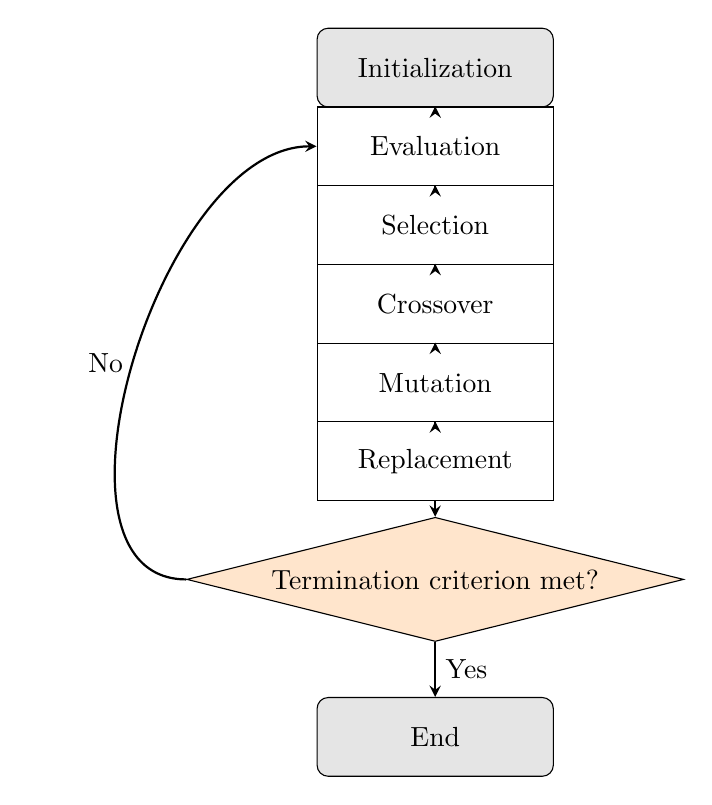
\begin{tikzpicture}[node distance=1.5cm]
            \usetikzlibrary{shapes.geometric, arrows.meta, positioning}

            \tikzstyle{startstop} = [rectangle, rounded corners, minimum width=3cm, minimum height=1cm,text centered, draw=black, fill=gray!20]
            \tikzstyle{process} = [rectangle, minimum width=3cm, minimum height=1cm, text centered, draw=black]
            \tikzstyle{decision} = [diamond, aspect=4, minimum width=2cm, text centered, draw=black, fill=orange!20]
            \tikzstyle{arrow} = [thick, ->, >=stealth]

            % Nodes
            \node (init) [startstop] {Initialization};
            \node (eval) [process, below of=init] {Evaluation};
            \node (select) [process, below of=eval] {Selection};
            \node (cross) [process, below of=select] {Crossover};
            \node (mutate) [process, below of=cross] {Mutation};
            \node (replace) [process, below of=mutate] {Replacement};
            \node (term) [decision, below of=replace, yshift=-0.5cm] {Termination criterion met?};
            \node (end) [startstop, below of=term, yshift=-1cm] {End};

            % Arrows
            \draw [arrow] (init) -- (eval);
            \draw [arrow] (eval) -- (select);
            \draw [arrow] (select) -- (cross);
            \draw [arrow] (cross) -- (mutate);
            \draw [arrow] (mutate) -- (replace);
            \draw [arrow] (replace) -- (term);
            \draw [arrow] (term) -- node[right] {Yes} (end);
            \draw [arrow] (term.west) .. controls +(-2,0) and +(-2,0) .. (eval.west) node[midway,left] {No};
        \end{tikzpicture}
    }
    \caption{Flowchart of a Genetic Algorithm.}
    \label{fig:ga_flowchart}
\end{figure}
        
        Genetic algorithms are versatile and can be applied to various optimization problems, including scheduling, routing, and function optimization. 
        Their ability to explore large solution spaces and adapt over time makes them powerful tools for solving complex problems.

